Lorem ipsum dolor sit amet, consectetur adipiscing elit. Sed consectetur, tortor ut cursus commodo, leo nisi lacinia orci, in consectetur odio ligula non lectus. Vestibulum vitae enim at libero feugiat finibus. Aliquam vitae malesuada odio. Nullam sed quam vel ex ultricies congue. Vivamus ac elit faucibus, sodales ex id, placerat quam. Quisque tristique dapibus nisl, in vestibulum leo malesuada sit amet. Proin ut augue semper, convallis tellus id, tincidunt nulla. Curabitur eu sollicitudin nisl. Morbi maximus diam eu neque volutpat faucibus. Phasellus non odio dui. Pellentesque fringilla ante at sem aliquam, sed consequat nisl pharetra. Nullam eu urna vel lectus efficitur maximus. Fusce ut ex eu purus rutrum tempor a sed lectus. Integer ultrices est elit, sed interdum ipsum efficitur in. Sed tristique, mauris eu tempor consectetur, ante massa fringilla risus, sed consectetur mi justo id nisi. Ut tempor luctus mauris sed fringilla. Vestibulum eu elit in turpis iaculis elementum. Aenean nec odio sit amet lorem elementum consequat. Vivamus condimentum metus a turpis consectetur luctus. Integer nec sem eu diam vestibulum tincidunt.

%-------------------------------------------------------------------------------------%
\section{Section 1: Title of the section} \label{sec:sec1}
Use acronyms like \gls{IoT}, and then if you use it again like \gls{IoT}, only the first one will appear in full form, and all subsequent usages will appear in short form. Some other abbreviations are \gls{LEO} and \gls{MEO}. You can also have acronyms like \gls{GEO}.

Lorem ipsum dolor sit amet, consectetur adipiscing elit. Sed consectetur, tortor ut cursus commodo, leo nisi lacinia orci, in consectetur odio ligula non lectus. Vestibulum vitae enim at libero feugiat finibus. Aliquam vitae malesuada odio. Nullam sed quam vel ex ultricies congue. Vivamus ac elit faucibus, sodales ex id, placerat quam. Quisque tristique dapibus nisl, in vestibulum leo malesuada sit amet. Proin ut augue semper, convallis tellus id, tincidunt nulla. Curabitur eu sollicitudin nisl. Morbi maximus diam eu neque volutpat faucibus. As shown in figure \ref{img:img1}.
\begin{figure}[t!]
 \centering
 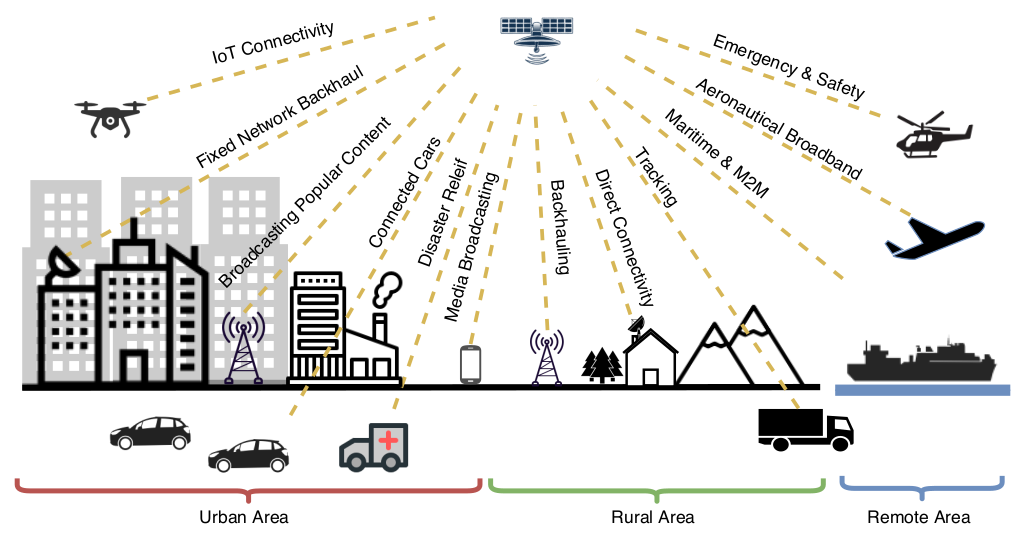
\includegraphics[scale=0.4]{figures/intro/1.png}
 \caption{Sample of an image put across full page width}
 \label{img:img1}
\end{figure}
Lorem ipsum dolor sit amet, consectetur adipiscing elit. Sed consectetur, tortor ut cursus commodo, leo nisi lacinia orci, in consectetur odio ligula non lectus. Vestibulum vitae enim at libero feugiat finibus. Aliquam vitae malesuada odio. Nullam sed quam vel ex ultricies congue. Vivamus ac elit faucibus, sodales ex id, placerat quam. Quisque tristique dapibus nisl, in vestibulum leo malesuada sit amet. Proin ut augue semper, convallis tellus id, tincidunt nulla. Curabitur eu sollicitudin nisl. Morbi maximus diam eu neque volutpat faucibus. Phasellus non odio dui.

Pellentesque fringilla ante at sem aliquam, sed consequat nisl pharetra. Nullam eu urna vel lectus efficitur maximus. Fusce ut ex eu purus rutrum tempor a sed lectus. Integer ultrices est elit, sed interdum ipsum efficitur in. Sed tristique, mauris eu tempor consectetur, ante massa fringilla risus, sed consectetur mi justo id nisi. Ut tempor luctus mauris sed fringilla. Vestibulum eu elit in turpis iaculis elementum. Aenean nec odio sit amet lorem elementum consequat. Vivamus condimentum metus a turpis consectetur luctus. Integer nec sem eu diam vestibulum tincidunt.

Nam sed mi eu tortor posuere sollicitudin eget ac lacus. Integer suscipit bibendum arcu, at semper leo faucibus non. In vulputate tortor eu neque ultrices, id feugiat tortor condimentum. Aenean vestibulum risus vitae nibh finibus, eget lobortis dolor placerat. Mauris in facilisis nisi. Proin congue auctor nisi, eu bibendum dui bibendum vitae. Fusce vitae arcu id lacus faucibus pretium. Donec quis turpis a metus eleifend finibus nec eget tortor. Curabitur interdum dui mauris, vitae finibus felis viverra in. Quisque eget est vitae nulla hendrerit iaculis. Phasellus pellentesque interdum elit, a finibus nunc iaculis a.
%------------------------------------------------
\section{Section 2: Example of a simple table} \label{sec:sec2}
\begin{figure}[t!]
 \centering
 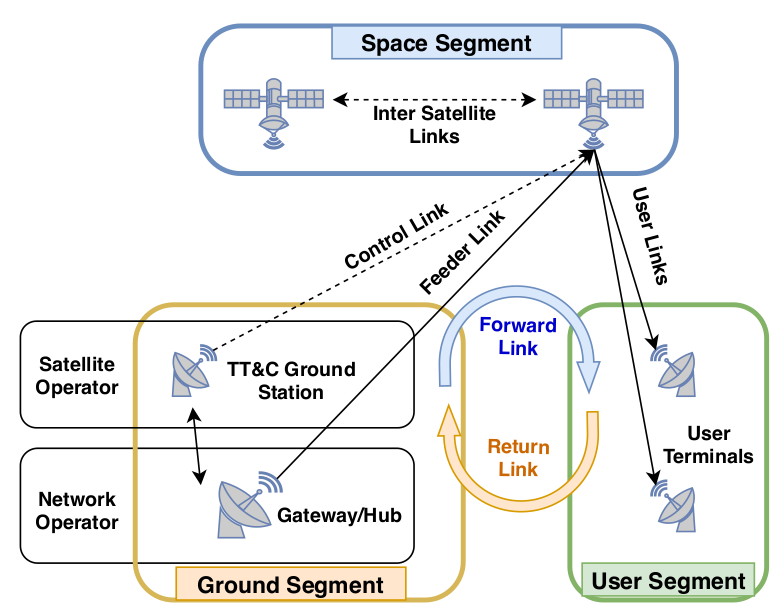
\includegraphics[scale=0.35]{figures/intro/3.png}
 \caption{Sample of a centered image put in single column}\label{img:img2}
\end{figure}
Lorem ipsum dolor sit amet, consectetur adipiscing elit. Sed consectetur, tortor ut cursus commodo, leo nisi lacinia orci, in consectetur odio ligula non lectus. Vestibulum vitae enim at libero feugiat finibus. Aliquam vitae malesuada odio. Nullam sed quam vel ex ultricies congue. Vivamus ac elit faucibus, sodales ex id, placerat quam. Quisque tristique dapibus nisl, in vestibulum leo malesuada sit amet. Proin ut augue semper, convallis tellus id, tincidunt nulla. Curabitur eu sollicitudin nisl. Morbi maximus diam eu neque volutpat faucibus. Phasellus non odio dui.

Pellentesque fringilla ante at sem aliquam, sed consequat nisl pharetra. Nullam eu urna vel lectus efficitur maximus. Fusce ut ex eu purus rutrum tempor a sed lectus. Integer ultrices est elit, sed interdum ipsum efficitur in. Sed tristique, mauris eu tempor consectetur, ante massa fringilla risus, sed consectetur mi justo id nisi. Ut tempor luctus mauris sed fringilla. Vestibulum eu elit in turpis iaculis elementum. Aenean nec odio sit amet lorem elementum consequat. Vivamus condimentum metus a turpis consectetur luctus. Integer nec sem eu diam vestibulum tincidunt Figure \ref{img:img2}

Nam sed mi eu tortor posuere sollicitudin eget ac lacus. Integer suscipit bibendum arcu, at semper leo faucibus non. In vulputate tortor eu neque ultrices, id feugiat tortor condimentum. Aenean vestibulum risus vitae nibh finibus, eget lobortis dolor placerat as shown in Figure \ref{fig:img3_a}, and Figure \ref{fig:img3}
%
\begin{figure}[t!]
\centering
    \subfigure[]{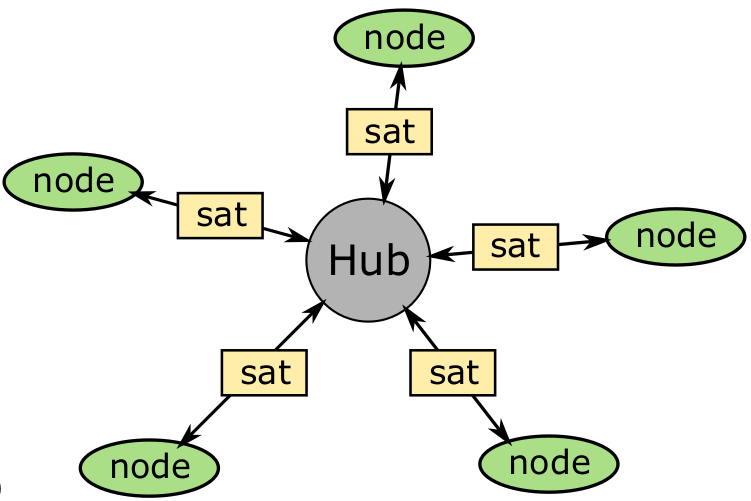
\includegraphics[width=0.45\textwidth]{figures/intro/4.png}\label{fig:img3_a}}\hfill
    \subfigure[]{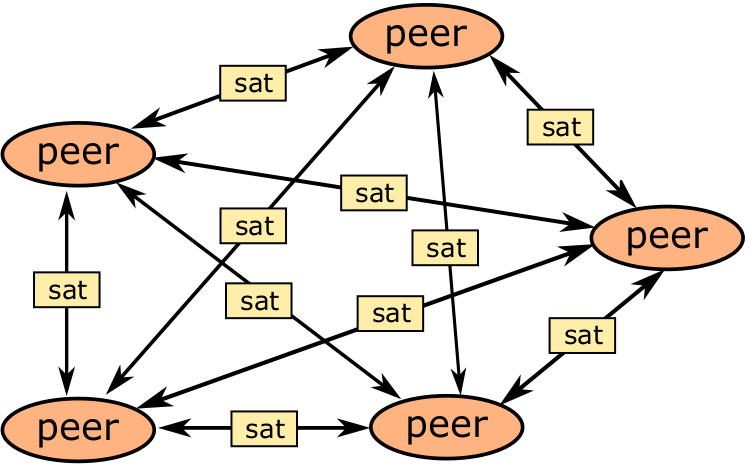
\includegraphics[width=0.45\textwidth]{figures/intro/5.png}\label{fig:img3_b}} 
    \caption{Sample of two parallel images put side-by-side (a) caption for first image (b) caption for second image}
    \label{fig:img3}
\end{figure}

%
\begin{table}[t!]
\centering
\caption{Sample of a simple table}
\vspace*{0.2cm}
\label{p1_tab:refScenarioApplications}
\begin{tabular}{|l|l|}
\hline
\textbf{Application/Use-Case} & \textbf{Reference   Scenario} \\
\hline \hline
A dense network of rural and urban air   quality monitoring & Scenario A, B, C, D, E \\\hline
Railway track condition monitoring & Scenario A, B, C, D \\\hline
Crowd monitoring (eg. large gatherings, stadiums, sports events) & Scenario E, F \\\hline
Smart agriculture applications – monitoring   and actuation & Scenario C, D, F \\\hline
Intrusion detection or emergency (SOS)   reporting & Scenario B, D, F\\
\hline
\end{tabular}
\end{table}
%
Based on the technical requirements, various applications, and use-cases are also mapped to these reference scenarios, as shown in Table. \ref{p1_tab:refScenarioApplications}.
%-------------------------------------------------------------------------------------%
\section{Section 3: Example of more complex looking table} \label{sec:sec3}
Pellentesque fringilla ante at sem aliquam, sed consequat nisl pharetra. Nullam eu urna vel lectus efficitur maximus. Fusce ut ex eu purus rutrum tempor a sed lectus. Integer ultrices est elit, sed interdum ipsum efficitur in. Sed tristique, mauris eu tempor consectetur, ante massa fringilla risus, sed consectetur mi justo id nisi. Ut tempor luctus mauris sed fringilla. Vestibulum eu elit in turpis iaculis elementum. Aenean nec odio sit amet lorem elementum consequat. Vivamus condimentum metus a turpis consectetur luctus. Integer nec sem eu diam vestibulum tincidunt
\begin{table}
    \centering
    \caption{Example of a more complex looking table}
    \vspace*{0.2cm}
    \label{p1_tab:link_budget}
    \resizebox{0.76\textwidth}{!}{%
    \begin{tabular}{|l|cccc|}
        \hline
            \textbf{Parameters} & \multicolumn{4}{c|}{\textbf{LEO - 600 km}} \\ \hline \hline
            
            Transmission mode & \multicolumn{2}{c|}{\textbf{DL}} & \multicolumn{2}{c|}{\textbf{UL}} \\ \hline
            
            Elevation angle {[}degree{]} & \multicolumn{1}{c|}{30} & \multicolumn{1}{c|}{90} & \multicolumn{1}{c|}{30} & 90 \\ \hline
            
            TX EIRP {[}dBW{]} & \multicolumn{2}{c|}{14} & \multicolumn{2}{c|}{-7} \\ \hline
            RX $G/T$ {[}dB/K{]} & \multicolumn{2}{c|}{-31.62} & \multicolumn{2}{c|}{- 18.6} \\ \hline
            
            BW$_\text{NB-IoT}$ {[}kHz{]} & \multicolumn{2}{c|}{180} & \multicolumn{2}{c|}{3.75/180} \\ \hline
            
            Free space path loss {[}dB{]} & \multicolumn{1}{c|}{159.10} & \multicolumn{1}{c|}{154.03} & \multicolumn{1}{c|}{159.10} & 154.03 \\ \hline
            
            Atmospheric loss {[}dB{]} & \multicolumn{4}{c|}{0.1} \\ \hline
            
            Shadowing margin {[}dB{]} & \multicolumn{4}{c|}{3} \\ \hline
            
            Scintillation loss {[}dB{]} & \multicolumn{4}{c|}{2.2} \\ \hline
            
            Polarization loss {[}dB{]} & \multicolumn{4}{c|}{3} \\ \hline
            
            Additional losses {[}dB{]} & \multicolumn{1}{c|}{3} & \multicolumn{1}{c|}{0} & \multicolumn{1}{c|}{3} & 0 \\ \hline
            
            \textbf{SNR {[}dB{]}} & \multicolumn{1}{c|}{\textbf{-11.97}} & \multicolumn{1}{c|}{\textbf{-3.9}} & \multicolumn{1}{c|}{\textbf{-3.14/-19.95}} & \textbf{4.86/-11.95} \\ \hline
    \end{tabular}%
    }
\end{table}

%-------------------------------------------------------------------------------------%
\section{Section 4: Example of simple algorithm} \label{sec:sec4}
A simple example of Algorithm \ref{algo:algo1}. Pellentesque fringilla ante at sem aliquam, sed consequat nisl pharetra. Nullam eu urna vel lectus efficitur maximus. Fusce ut ex eu purus rutrum tempor a sed lectus. Integer ultrices est elit, sed interdum ipsum efficitur in. Sed tristique, mauris eu tempor consectetur, ante massa fringilla risus, sed consectetur mi justo id nisi. Ut tempor luctus mauris sed fringilla. Vestibulum eu elit in turpis iaculis elementum. Aenean nec odio sit amet lorem elementum consequat. Vivamus condimentum metus a turpis consectetur luctus. Integer nec sem eu diam vestibulum tincidunt
\begin{algorithm}
\caption{Example of a basic algorithm}\label{algo:algo1}
    \begin{algorithmic}
    \State \textbf{Initialize:} No. of channel realizations L
    \State \textbf{Initialize:} $U, S, r_{\text{min}}, \theta_0$, and other link parameters
    \State \textbf{Generate:} Channel $\mathbf{H}_{U,S,\text{L}}$, $\mathbf{G}_{S,\text{L}}$, Range $\mathbf{R}_{U,S,\text{L}}$
        \For{$l = 1 \text{ to } U$}
            \State \textbf{Compute}: $\gamma_{us}^{(l)} \quad \forall \, u \notin \mathbf{D}[\,l-1\,]$
            %%\vspace4pt}
            \State \textbf{Perform:} MRC:  $\gamma_u^{(l)} \gets \sum_{s=1}^{S} \gamma_{us}^{(l)} \quad \forall \, u \notin \mathbf{D}[\,l-1\,].$
            %%\vspace4pt}
            \If {$l=1$}
                \State CM: $\gamma_u \gets \texttt{sort}\, \gamma_u^{(1)}$
                \State SIC: $\gamma_{\mathbf{D}\{l\}}^{(l)} \gets \max\limits_{u} \gamma_{u}^{(l)}$
            \ElsIf {$l>1 \, \& \, \gamma_{\mathbf{D}\{l-1\}}^{(l-1)} > \gt$}
                \State SIC: $\gamma_{\mathbf{D}\{l\}}^{(l)} \gets \max\limits_{u, u \notin \mathbf{D}[\,l-1\,]} \gamma_{u}^{(l)}$
            \Else
                \State SIC: $\gamma_{\mathbf{D}\{l\}}^{(l)} \gets 0$
            \EndIf
            %%\vspace4pt}
            \State \textbf{Remove:} Entries of $\mathbf{D}[l]$ from $\mathbf{H}$, $\mathbf{G}$ and $\mathbf{R}$    
        \EndFor
    \end{algorithmic}
\end{algorithm}

Lorem ipsum dolor sit amet, consectetur adipiscing elit. Sed consectetur, tortor ut cursus commodo, leo nisi lacinia orci, in consectetur odio ligula non lectus. Vestibulum vitae enim at libero feugiat finibus. Aliquam vitae malesuada odio. Nullam sed quam vel ex ultricies congue. Vivamus ac elit faucibus, sodales ex id, placerat quam. Quisque tristique dapibus nisl, in vestibulum leo malesuada sit amet. Proin ut augue semper, convallis tellus id, tincidunt nulla. Curabitur eu sollicitudin nisl. Morbi maximus diam eu neque volutpat faucibus. Phasellus non odio dui.

Pellentesque fringilla ante at sem aliquam, sed consequat nisl pharetra. Nullam eu urna vel lectus efficitur maximus. Fusce ut ex eu purus rutrum tempor a sed lectus. Integer ultrices est elit, sed interdum ipsum efficitur in. Sed tristique, mauris eu tempor consectetur, ante massa fringilla risus, sed consectetur mi justo id nisi. Ut tempor luctus mauris sed fringilla. Vestibulum eu elit in turpis iaculis elementum.

\textbf{Example text to create citations:}
\begin{enumerate}
    \item \textbf{Conference:} The work done in \cite{conference1} is very influential in the field of so and so.
    \item \textbf{Journal:} Also, in \cite{journal1}, so and so work has been done.
    \item \textbf{Book:} Also, in \cite{book1}, so and so work has been done.
    \item \textbf{Webpage with link:} The report is available at \cite{link1}.
\end{enumerate} 